\begin{figure*}[t]
    \centering
    \begin{tikzpicture}[font={\tiny},]
         %% CNN branch
        \node(input) at (-5.5, 0) {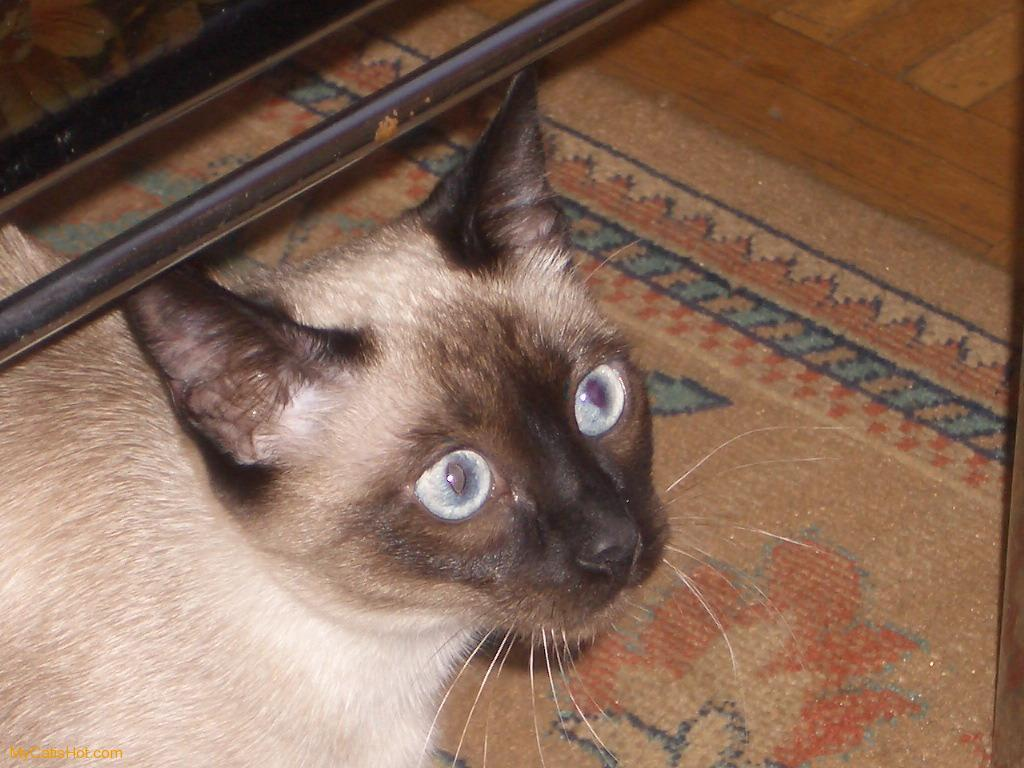
\includegraphics[width=.1\textwidth]{Images/Method/input.jpg}};
        \node[] at (input.north) {\footnotesize Input image $\vx$};
        \node[draw, trapezium, rotate=-90,trapezium angle=75, align=center] (res0) at (-3.5,0) {\rotatebox{90}{\parbox{1.0cm}{\centering{\footnotesize Res-0}\\$d_0$}}};
        \node[draw, trapezium, rotate=-90,trapezium angle=75, align=center] (res1) at (-1.5,0) {\rotatebox{90}{\parbox{1.0cm}{\centering{\footnotesize Res-1}\\$d_1$}}};
        \node[draw, trapezium, rotate=-90,trapezium angle=75, align=center] (res2) at (0.5,0) {\rotatebox{90}{\parbox{1.0cm}{\centering{\footnotesize Res-2}\\$d_2$}}};
        \node[draw, trapezium, rotate=-90,trapezium angle=75, align=center] (res3) at (2.5,0) {\rotatebox{90}{\parbox{1.0cm}{\centering{\footnotesize Res-3}\\$d_3$}}};
        \node[draw, trapezium, rotate=-90,trapezium angle=75, align=center] (res4) at (4.5,0) {\rotatebox{90}{\parbox{1.0cm}{\centering{\footnotesize Res-4}\\$d_4$}}};
        \node[](empt1) at (6.5, 0){};
        \node[draw, rotate=90, align=center] (class) at (7,0) {\footnotesize Classifier};
        \node(logit) at (7.75, 0) {\small$\vy$};
        %%% CLS stream
        \node[align=center](clsin) at (-4, -1.5) {{\footnotesize[CLS],}\\$d_{cls}$};
        \node[draw, align=center](CA0) at (-2.5, -1.5) {{\footnotesize CA-0}, \\$d_0$};
        \node[draw, align=center](CA1) at (-0.5, -1.5) {{\footnotesize CA-1}, \\$d_1$};
        \node[draw, align=center](CA2) at (1.5, -1.5) {{\footnotesize CA-2}, \\$d_2$};
        \node[draw, align=center](CA3) at (3.5, -1.5) {{\footnotesize CA-3}, \\$d_3$};
        \node[draw, align=center](CA4) at (5.5, -1.5) {{\footnotesize CA-4}, \\$d_4$};

        %% CNN backbone
        \node(empt0) at (-4.65, 0) {};
        \draw[->] (empt0.center) -- node {} (res0);
        \draw[->] (res0) -- node {} (res1);
        \draw[->] (res1) -- node {} (res2);
        \draw[->] (res2) -- node {} (res3);
        \draw[->] (res3) -- node {} (res4);
        \draw[->] (res1) -- node {} (res2);
        \draw[->] (res2) -- node {} (res3);
        \draw[->] (res3) -- node {} (res4);
        \draw[->, blue, dashed] (res4) -- node {\blue{\normalsize//}} (class);
        \node[](GAP) at (6,0.25) {\footnotesize\blue{$\gap$}};
        \draw[->] (class) -- node {} (logit);
        %% CLS Stream
        \draw[->] (clsin) -- node {} (CA0);
        \draw[dashed, ->] (res0.north) -|node {} (CA0);
        \draw[->] (CA0) -- node {} (CA1);
        \draw[dashed, ->] (res1.north) -|node {} (CA1);
        \draw[->] (CA1) -- node {} (CA2);
        \draw[dashed, ->] (res2.north) -|node {} (CA2);
        \draw[->] (CA2) -- node {} (CA3);
        \draw[dashed, ->] (res3.north) -|node {} (CA3);
        \draw[->] (CA3) -- node {} (CA4);
        \draw[dashed, ->] (res4.north) -|node {} (CA4);
        \draw[-] (CA4.east) -| node {} (empt1.center);
        \draw[->] (empt1.center) -- node {} (class);
        % \path[->] (CA4.east) edge[bend right,left] node {} (class.north);
        % \path [->] (B) edge[bend right=60] node {$1$} (E);
    \end{tikzpicture}
    \caption{\emph{Cross Attention Stream applied to ResNet-based architectures.} Given a CNN backbone $f(\cdot)$, we replace global average pooling as a representation for the classifier, with  the introduction of a global representation [CLS] learned with the inclusion of the cross attention  stream. For a given layer $\ell$ we update our [CLS] token $Q_\ell$; by computing its scaled cross attention with the feature maps $F_\ell$, that are then projected to the channel dimension in the following stage, using a dense layer parametrized by $w_\ell$.}
    \label{fig:fig_method}
\end{figure*}
